
\section{Einführung\hfill\textnormal{\emph{Löbel}}}
Die Domäne Rettungsrobotik verfügt über sehr vielversprechende wirtschaftliche Aspekte. Menschliche Rettungskräfte sind bei Katastrophen Szenarien eine knappe Ressource. Ein einzelner Bediener sollte daher idealerweise eine Vielzahl von Robotern überwachen. Beim Einsatz solcher Rettungsroboter ist ein hohes Maß an Autonomie gefordert. Sie begegnen einer Vielzahl unbekannter Objekte. Sie sollten in der Lage sein, Objekte oder ihre Umgebung zu erkennen und spezifiziert darauf zu reagieren. Es gibt zwei Entwicklungsziele, die schwer zu kombinieren sind. Zum einen ist für die Umsetzung eines autonomen Systems High-Technology notwendig. Zum anderen gibt es den Bedarf möglichst einfache und kostengünstige Systeme zu entwickeln \cite{birk2006rescue}. Bei diesem Projekt des "Rescue Robots“ liegt der Hauptfokus zunächst auf der Umsetzung der Funktionalität.

\hfill August 27, 2020

\subsection{Produktübersicht}
Der Rescue Robot soll auf einem Industriegelände, auf dem es eine Explosion gab, eingesetzt werden. Auf dem Gelände können sich noch Personen befinden, die eventuell verletzt sind. Dies bedeutet, dass auch ein Rettungsdienst vor Ort sein muss. Dieser soll über den Rescue Robot mit verletzten Personen kommunizieren können. In Abb.\ref{Produktuebersicht} wird dargestellt, in welchem Kontext der Rescue Robot seinen Einsatz findet.

\begin{figure}[H]
  \centering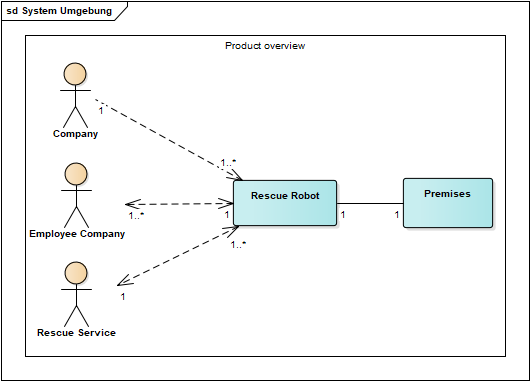
\includegraphics[width=1\linewidth]{Produktuebersicht.png}
  \caption{Produktuebersicht}
  \label{Produktuebersicht}
\end{figure}

\subsection{Systemumgebung}
Der Rescue Robot soll das Firmengelände autonom erkunden können. Hierfür soll er Radiosignalen folgen können. Diese werden von Funktürmen auf dem Firmengelände gesendet. Das Firmengelände ist durch Mauern begrenzt. Durch die Explosion befinden sich auf dem Gelände unter anderem Gesteinsbrocken, welche umfahren werden müssen. Aber auch Gegenstände, die je nach radioaktiver Strahlung, aufgesammelt werden müssen. Das Firmengelände besteht hauptsächlich aus festem Untergrund. Jedoch ist durch die Explosion auch ein Wasserloch entstanden, welches der Roboter überqueren können soll. Zusätzlich wird die Sicht durch Nebel oder Rauch erschwert. Außerdem können sich verletzte Personen auf dem Gelände befinden. In Abb.\ref{Systemumgebung} ist die Systemumgebung, das Firmengelände "Premises" als Klassendiagramm dargestellt. 

\begin{figure}[H]
  \centering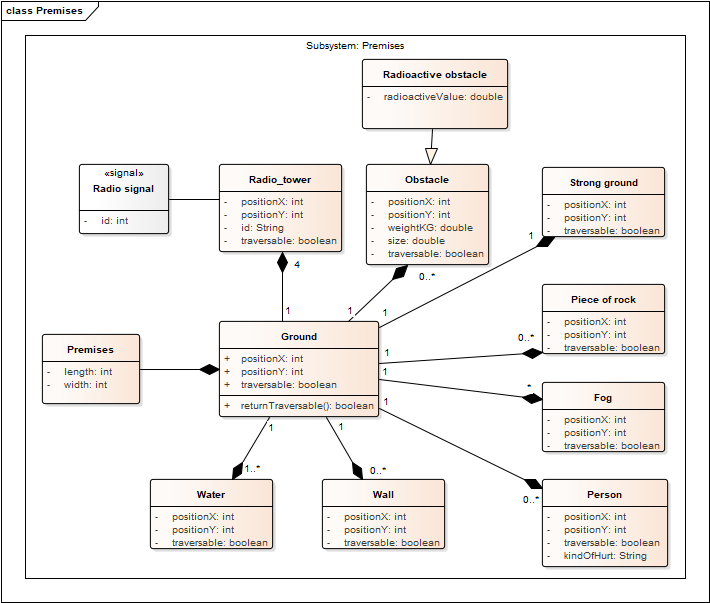
\includegraphics[width=1\linewidth]{Premises.png}
  \caption{Systemumgebung}
  \label{Systemumgebung}
\end{figure}

\subsection{Anforderungen}  \label{sec:reqs}
Aus dem beschriebenen Szenario lassen sich folgende Anforderungen festhalten, siehe Abb.\ref{Requirements}.

\begin{figure}[H]
  \centering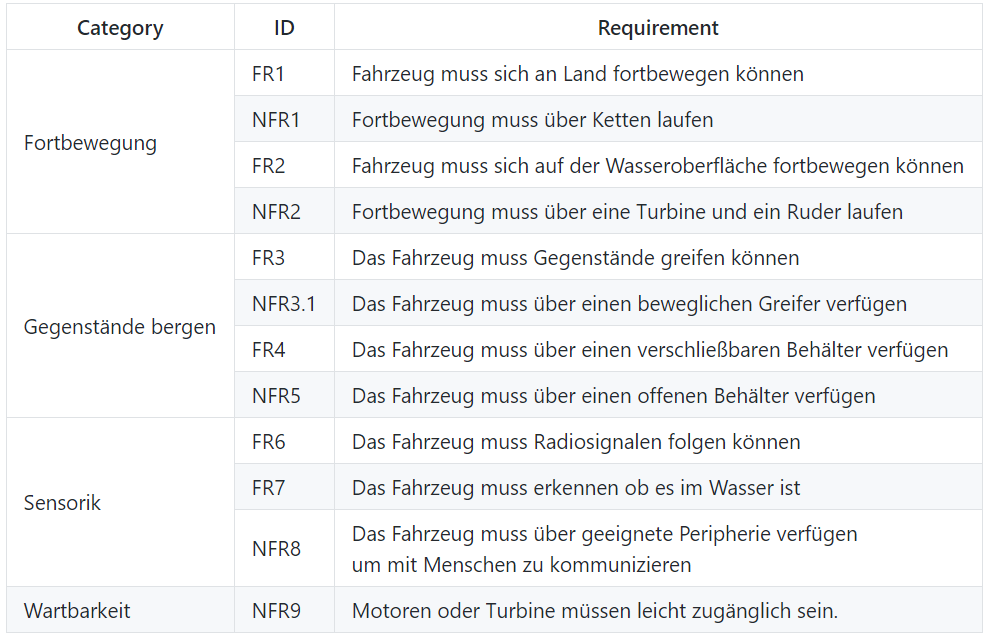
\includegraphics[width=1\linewidth]{Requirements.png}
  \caption{Requirements}
  \label{Requirements}
\end{figure}

Die funktionalen Anforderungen ergeben folgendes Use Case Diagram (Abb.\ref{UseCase}), welche das System beschreiben. Der Rescue Robot soll sich sowohl an Land als auch im Wasser fortbewegen können. Hierzu muss er mittels eines Sensors erkennen können, ob er sich an Land oder im Wasser befindet. Zudem muss der Rescue Robot Radiosignale empfangen und diesen folgen können. Trifft der Roboter auf radioaktive Objekte sollen diese eingesammelt werden. Dazu muss der Roboter über einen beweglichen Greifer verfügen und greifen können. Außerdem soll mit Personen, die sich noch auf dem Gelände befinden, kommuniziert werden können. Der Roboter muss deshalb über die geeignete Peripherie wie Kamera, Lautsprecher und Mikrophon verfügen.

\begin{figure}[H]
  \centering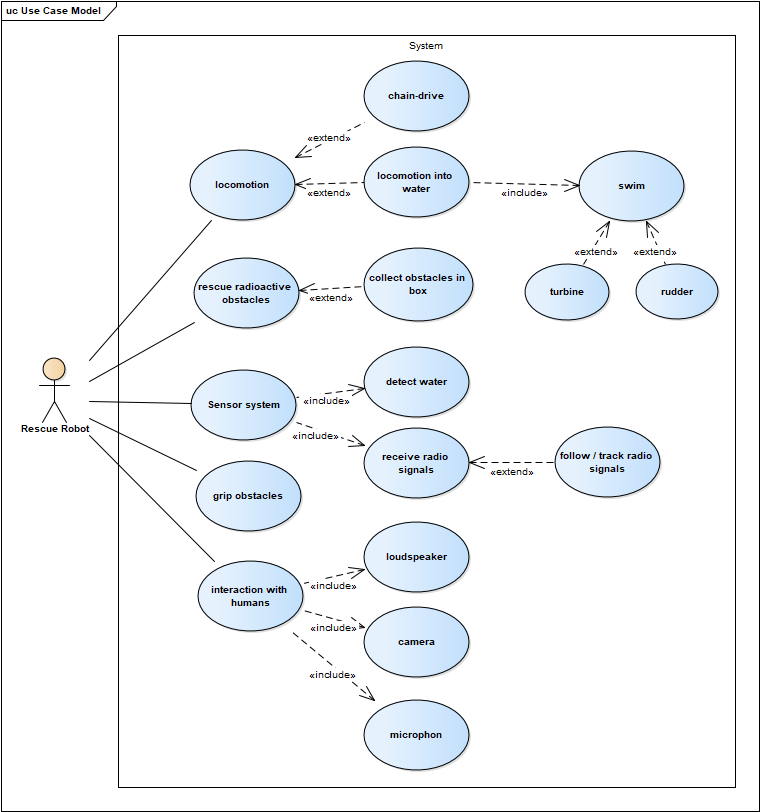
\includegraphics[width=1\linewidth]{Use Case Model.png}
  \caption{Use Case Diagram}
  \label{UseCase}
\end{figure}

